\label{section:gimbal_controller_results}

As stated in Section \ref{subsection:aiming_the_camera}, the main job of the gimbal controller is to aim the camera directly at the landing platform. It does this by using 2 PID controllers - one on its pitch angle and one on its yaw angle - to control its 2 degrees of freedom. Initially, PD controllers were used for this purpose, but they were inadequate as the simulated gimbal has spring forces which tend to keep the gimbal's positions at their original points. As the magnitude of the pitch or yaw angles increases, the force required to further increase the angle's magnitude increases. Over time, a small integral gain helps correct the error caused by this change in required force. Table \ref{tab:gimbal_controller_pid_gains} shows the gains for the gimbal PID controllers.

\begin{table}[ht]
    \centering
    \begin{tabular}{|c|c|c|c|}
    \hline
        Controller & $k_p$ & $k_i$ & $k_d$ \\\hline
        Pitch & 0.25 & 0.1 & 0.025 \\\hline
        Yaw & 0.25 & 0.1 & 0.025 \\\hline
    \end{tabular}
    \caption{Gimbal controller PID gains.}
    \label{tab:gimbal_controller_pid_gains}
\end{table}

The $x$ and $y$ components of the un-transformed landing platform pose comprise the input for target angle calculation, and these target angles are used as the set points for the PID controllers. The $x$ and $y$ components are scaled by a factor inversely proportional to the $z$ component in order to allow the PID controllers to function in a stable way over a variety of distances. If the $x$ and $y$ components are used without scaling, the PID controllers wildly overshoot at long distances and undershoot at short distances. Figures \ref{subfig:x_displacement} and \ref{subfig:y_displacement} show the performance of the gimbal controller during 10 landings. In both figures, each line represents a single attempt to aim camera over the course of the landing. Time $t=0$ represents that time of first recognition of the landing platform. At about 30 seconds in each landing sequences, the drone has made contact with the landing platform. The graph continues in time until the drone disarms, completing the landing. Figure \ref{subfig:x_displacement} shows that, after some oscillation, the yaw of the gimbal is adjusted so that the marker is in the center of the camera's view in the $x$ direction. Figure \ref{subfig:y_displacement} shows similar results with regards to the gimbal's pitch, but with an added, temporary bias during which time the gimbal is pointed slightly lower than the landing platform. This is because, when the drone is close to the landing pad, the April Tag marker is almost directly in front of the drone and therefore the spring resistance in the gimbal is high. The error is eventually corrected by the integral gain and the marker becomes centered in the $y$ direction of the camera frame. Centering of the landing platform in the camera's field of view is represented by the convergence of each line to 0. However, even though the ideal goal of the gimbal controller is to keep the landing platform centered in this way, it is only critical that it must keep the landing platform in the camera's field of view throughout a variety of orientations and displacements. These figures show that the gimbal controller does accomplish this goal.

\begin{figure}[ht]
    \centering
    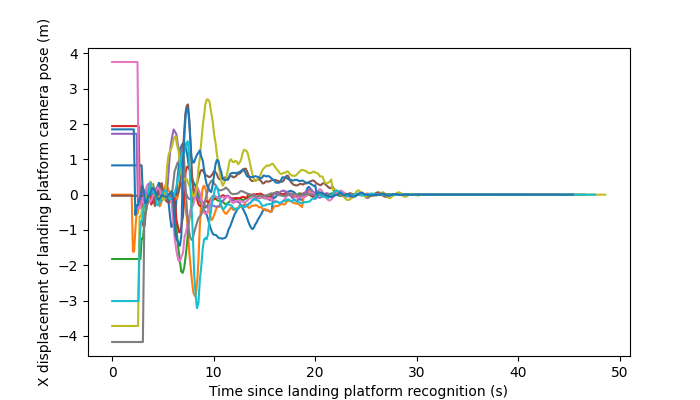
\includegraphics[width=0.7\textwidth]{images/x_displacement.png}
    \caption[Landing platform $x$ displacement in camera frame versus time.]{Landing platform $x$ displacement in camera frame versus time. Each line represents a single attempt to aim the camera during landing.}
    \label{subfig:x_displacement}
\end{figure}

\begin{figure}[ht]
    \centering
    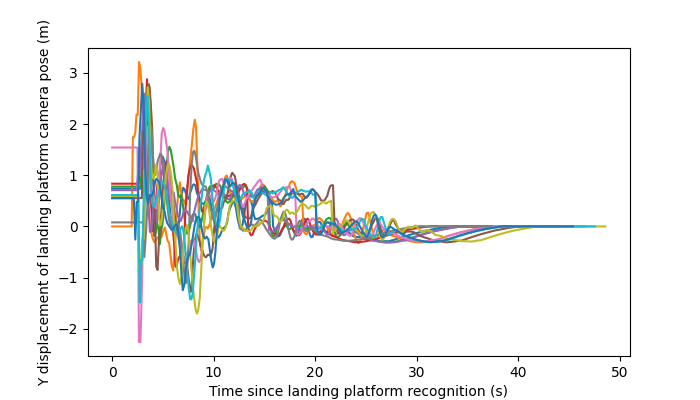
\includegraphics[width=0.7\textwidth]{images/y_displacement.png}
    \caption[Landing platform $y$ displacement in camera frame versus time.]{Landing platform $y$ displacement in camera frame versus time. Each line represents a single attempt to aim the camera during landing.}
    \label{subfig:y_displacement}
\end{figure}

% \begin{figure}[ht]
%     \centering
%     \begin{subfigure}[b]{0.47\textwidth}
%         \centering
%         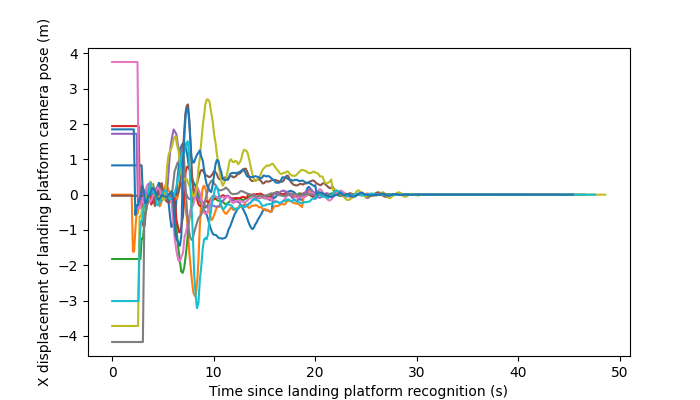
\includegraphics[width=\textwidth]{images/x_displacement.png}
%         \caption{Landing platform X displacement in camera frame.}
%         \label{subfig:x_displacement}
%     \end{subfigure}
%     \begin{subfigure}[b]{0.47\textwidth}
%         \centering
%         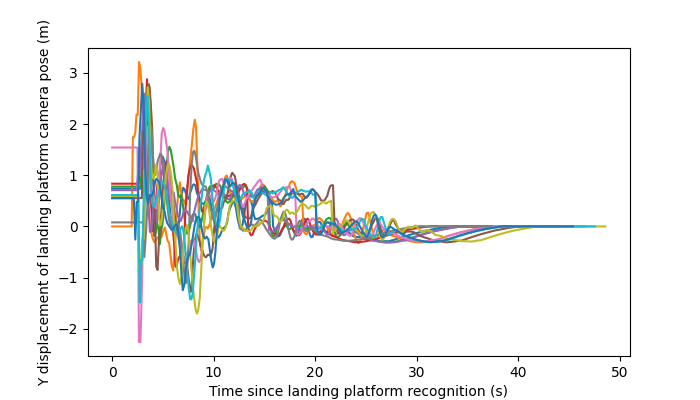
\includegraphics[width=\textwidth]{images/y_displacement.png}
%         \caption{Landing platform Y displacement in camera frame.}
%         \label{subfig:y_displacement}
%     \end{subfigure}
%     \caption{Time versus linear displacement in X and Y directions for landing platform pose in camera frame.}
%     \label{subfig:gimbal_x_y_displacement}
% \end{figure}

The pose of the landing platform in the $z$ direction behaves differently, in that it converges to some non-zero distance representing the depth of the landing platform in the camera frame. As the drone approaches the landing platform, this depth of course decreases to near-zero as the drone lands.

\begin{figure}[ht]
    \centering
    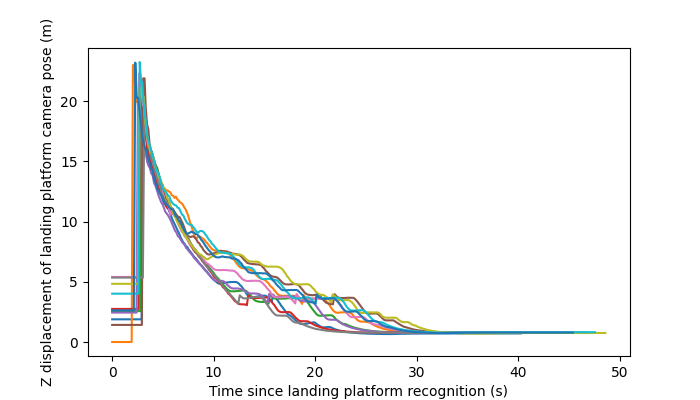
\includegraphics[width=0.7\textwidth]{images/z_displacement.png}
    \caption[Landing platform $z$ displacement in camera frame versus time.]{Landing platform $z$ displacement in camera frame versus time. Each line represents a single attempt to aim the camera during landing.}
    \label{fig:gimbal_z_displacement}
\end{figure}